 \subsection{Pannello}\label{archPannello}
Per rendere lo sviluppo più semplice, e garantire la manutenibilità del codice il team ha optato per un approccio modulare. In questo modo, avendo moduli separati con compiti distinti, sarà più semplice modificarne o estenderne il comportamento senza dover necessariamente modificare la base comune.\\
%  Il seguente diagramma delle classi mostra le relazioni tra i vari moduli. 


\subsubsection{UML}
\begin{figure}[H]
	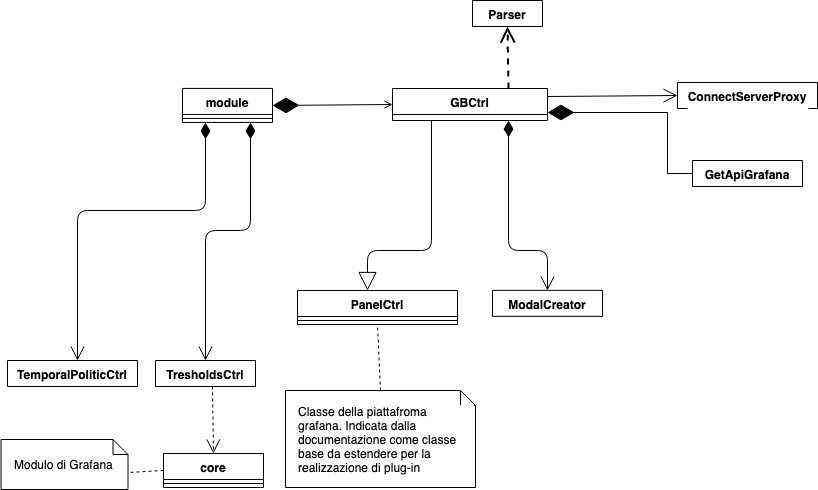
\includegraphics[width=\textwidth]{./images/plugin_non_espanso.png}
	\caption{Diagramma delle classi del Pannello}
\end{figure}

\begin{itemize}
	\item \textbf{GBCtrl}: è il modulo principale del plug-in, considerato come \textit{"main"} dall'ecosistema grafana, viene utilizzato per inizializzare l'intero panello; 
	\item \textbf{TemporalPolicyCtrl}: è il modulo che si occupa di gestire ed impostare le politiche temporali all'interno del pannello;
	\item \textbf{ThresholdsCtrl}: è il modulo che si occupa di gestire ed impostare le soglie per il monitoraggio;
	\item \textbf{Parser}: è il modulo che si occupa di controllare e interpretare la rete bayesiana in input, in formato \textit{JSON};
	\item \textbf{ConnectServer}: è il modulo che si occupa di inoltrare le richieste al Server;
	\item \textbf{ModalCreator}: è il modulo che si occupa di visualizzare le finestre che permettono l'interazione con l'utente;
	\item \textbf{ModalCreator}: è il modulo che si occupa della creazione e visualizzazione dinamica di finestre, le quali permettono l'interazione con l'utente: 
	\item \textbf{GetAPIGrafana}: è il modulo che si occupa di interagire con le API di \textit{Grafana} per ottenere i dati relativi alle sorgenti dati.
\end{itemize}

\subsubsection{Descrizione delle Classi e dei Metodi del Pannello}\label{classiPannelloDescrizione}
	
	  \paragraph{GBCtrl} 
		\begin{itemize}
			\item \textbf{resetData()} : metodo usato per riportare lo stato del pannello a prima che venga caricata una rete. Viene usato quando si deve caricare una nuova rete per eliminare le precedenti impostazioni;
			\item \textbf{resetTresholds()} : metodo usato per preparare il pannello a salvare le soglie di una nuova rete. Elimina le soglie precedenti e imposta il dizionario coi nodi della nuova rete;
			\item \textbf{checkIfAtLeastOneTresholdDefined()} : controlla se l'utente ha definito almeno una soglia, viene invocato al momento dell'inizio del monitoraggio;
			\item \textbf{deleteLinkToFlush(node)} : cancella il collegamento di un nodo ad un flusso dati e ne cancella le soglie. Viene richiamato quando l'utente clicca sul pulsante "Scollega Nodo";
			\item \textbf{freeAllFlushes()} : elimina tutti i collegamenti ai flussi e riaggiunge i flussi a quelli disponibili da scegliere. Viene invocato dal metodo \textit{resetData()};
			\item \textbf{getDatabases()} : metodo invocato al momento della creazione del pannello per ottenere da \textit{Grafana} i database disponibili;
			\item \textbf{getConnectionToDb()} : metodo che crea l'oggetto per ottenere i dati sui flussi dal database. Viene invocato al momento del collegamento al database;
			\item \textbf{checkIfConnectableToDB()} : metodo che verifica se ci si possa connettere al database selezionato, verificando: che la rete non sia sotto monitoraggio, sia stato selezionato un database e che il database selezionato sia di tipo influxdb;
			\item \textbf{getFlushes()} : metodo usato per ottenere i flussi dal database selezionato. Viene invocato quando ci si collega al database  o si carica una rete salvata nel Server;
			\item \textbf{connectToDB()} : metodo che effettua il collegamento al database. Viene invocato quando l'utente preme il pulsante "Conferma" per selezionare il database;
			\item \textbf{showTresholdModal(node)} : metodo invocato quando l'utente preme sul nome di un nodo. Fa apparire la modal per impostare le soglie;
			\item \textbf{selectTemporalPolicy()} : metodo invocato quando l'utente preme sul pulsante "Imposta" che fa apparire la modal per impostare la politica temporale;
			\item \textbf{visualizeMonitoring()} : metodo invocato quando l'utente preme il pulsante "Visualizza Monitoraggi Attivi", che fa cambiare la schermata per visualizzare i monitoraggi;
			\item \textbf{visualizeSettings()} : metodo invocato quando l'utente preme il pulsante "Visualizza Impostazioni", per tornare alla schermata delle impostazioni della rete;
			\item \textbf{splitMonitoringNetworks()} : metodo invocato quando vengono richieste le reti al Server. Si preoccupa di capire quali sono sotto monitoraggio e di suddividerle correttamente;
			\item \textbf{requestNetworks()} : metodo invocato ogni volta che viene salvata una rete sul Server e quando ci si collega ad esso. Richiede la lista delle reti al Server;
			\item \textbf{tryConnectServer()} : metodo per provare a vedere se il Server è online su porta e ip specificati. Viene invocato quando l'utente preme sul tasto "Connetti" da Server Settings;
			\item \textbf{checkIfNetworkIsDeletable(net)} : metodo che viene invocato quando l'utente preme sul tasto "Elimina" per eliminare una rete. Richiede al Server che venga eliminata la rete selezionata;
			\item \textbf{calculateSeconds(temp)} : metodo per calcolare i secondi totali della politica temporale. Viene usato dal metodo changeNetworkToVisualizeMonitoring() per impostare la politica di refresh delle probabilità;
			\item \textbf{deleteProbRefresh()} : metodo usato per eliminare l'intervallo di refresh delle probabilità. Viene invocato quando l'utente ritorna alla schermata delle impostazioni delle reti;
			\item \textbf{updateProbs()} : metodo invocato per aggiornare il disegno delle probabilità della rete. Viene invocato ad intervalli regolari stabiliti dalla politica temporale della rete;
			\item \textbf{changeNetworkToVisualizeMonitoring()} : metodo invocato quando l'utente seleziona una nuova rete di cui visualizzare le probabilità. Imposta il timer di refresh delle probabilità e aggiorna il disegno della rete;
			\item \textbf{buildDataToSend()} : metodo invocato quando bisogna salvare una rete sul Server. Costruisce il pacchetto contenente tutti i dati necessari da salvare;
			\item \textbf{loadNetworkToServer(net)} : metodo usato per salvare una rete sul Server;
			\item \textbf{saveActualChanges()} : metodo invocato quando viene caricata una rete. Verifica se era già presente una rete e se essa abbia bisogno di essere salvata sul Server. In caso positivo la salva prima di caricare quella nuova;
			\item \textbf{requestNetworkToServer(net)} : metodo invocato quando l'utente preme il pulsante "Apri" per caricare una rete salvata nel Server. Si occupa di caricare nel pannello le informazioni della rete e di collegarsi al database corretto;
			\item \textbf{loadNetworkFromSaved(net)} : metodo usato quando l'utente carica una rete da quelle salvate. Si occupa di assegnare le variabili;
			\item \textbf{loadNetwork(data)} : metodo invocato quando l'utente clicca sul pulsante per confermare la rete da caricare dalla memoria locale. Si preoccupa verificare che la rete sia corretta e di inizializzarla;
			\item \textbf{panelPath()} : metodo per ottenere il percorso del pannello;
			\item \textbf{checkIfCanStartComputation()} : metodo che verifica se l'utente ha correttamente impostato i parametri per far partire la computazione;
			\item \textbf{startComputation()} : metodo invocato quando l'utente preme sul pulsante "Avvia Monitoraggio". Esso fa partire la computazione e salva la rete nel Server;
			\item \textbf{closeComputation()} : metodo invocato quando l'utente preme sul pulsante "Interrompi Monitoraggio" per interrompere il monitoraggio.
	\end{itemize}
	  \paragraph{TemporalPolicyCtrl} 
			\begin{itemize}
				\item	\textbf{checkCorrectData()} : metodo che verifica la correttezza dei dati inseriti per la politica temporale;
				\item \textbf{setConfirmationToTrue()} : metodo invocato quando l'utente preme sul tasto "Conferma" dalla modal della politica temporale. Verifica che sia stata impostata correttamente e lo notifica al pannello, facendo anche sparire la modal;
				\item \textbf{setConfirmationToFalse()} : metodo invocato quando l'utente modifica la politica temporale  per notificare al pannello che al momento non è valida.
	\end{itemize}
				  \paragraph{TresholdsCtrl}
			\begin{itemize}
				\item \textbf{checkIfTherIsAtLeastOneTreshold(node)} : verifica che l'utente abbia impostato almeno una soglia. Viene invocato dal metodo \textit{confirmTresholdsChanges(node)} per verificare che l'utente abbia definito almeno una soglia;
				\item \textbf{checkNotRepeatedTresholds(node)} : verifica che l'utente non abbia definito soglie ripetute. Viene invocato dal metodo \textit{confirmTresholdsChanges(node)};
				\item \textbf{splitForSign(node)} : divide le soglie per segno. Viene invocato per verificare che non ci siano conflitti tra le soglie;
				\item \textbf{setError(value1, value2, sign1, sign2)} : metodo invocato da tutti gli altri metodo qual ora vi sia un errore. fa apparire una modal con l'errore;
				\item \textbf{checkConflictMin(min, maj, maje)} : verifica che non ci siano conflitti tra le soglie "<" con le soglie ">" e ">=". Viene in vocato dal metodo\textit{checkConflicts(data)};
				\item \textbf{checkConflictMine(mine, maj, maje)} : verifica che non ci siano conflitti tra le soglie "<=" con le soglie ">" e ">=". Viene in vocato dal metodo\textit{checkConflicts(data)};
				\item \textbf{checkConflictSameSign(arr1, arr2, sign1, sign2)} : verifica che non ci siano conflitti tra le soglie con lo stesso segno. Viene in vocato dal metodo\textit{checkConflicts(data)};
				\item \textbf{checkConflicts(data)} : si occupa di invocare tutti i metodi per verificare la presenza di conflitti tra le soglie. Viene invocato dal metodo \textit{confirmTresholdsChanges(node)};
				\item \textbf{associate(node)} : crea l'associazione tra il nodo e il flusso attualmente selezionato. Viene invocato dal metodo \textit{confirmTresholdsChanges(node)}.
				\item \textbf{confirmTresholdsChanges(node)} : metodo invocato quando l'utente preme sul tasto "Conferma" dalla modal della politica temporale. Invoca tutti i metodi per verificare la correttezza delle soglie e crea le associazioni qual ora necessario;
				\item \textbf{addTreshold(node, state)} : metodo invocato quando l'utente preme un tasto per aggiungere una soglia al nodo. Aggiunge la soglia relativa allo stato a cui si riferisce;
				\item \textbf{deleteTreshold(node, name)} : metodo invocato quando l'utente preme su un tasto "Remove" dalla modal delle soglie. Rimuove la soglia corrispondente;
				\item \textbf{setNotLinked(node)} : rimuove il collegamento tra il nodo e il flusso. Viene invocato quando l'utente esegue una qualsiasi azione diversa dal confermare le soglie dalla modal delle soglie;
				\item \textbf{setLinked(node)} : imposta il nodo come collegato. Viene invocato dal metodo \textit{confirmTresholdsChanges(node)};
			\end{itemize}
		
		 \paragraph{Parser} 
			\begin{itemize}
				\item \textbf{validateNet()} : invoca tutti i metodi per verificare la correttezza della rete;
				\item \textbf{checkMinimumFields()} : verifica che il file \textit{.JSON} abbia il numero corretto di campi, i quali devono avere anche il nome corretto;
				\item \textbf{checkNamedNodes(data, field)} : verifica che il campo data abbia il corretto numero di linee e che esse abbiano il nome giusto;
				\item \textbf{checkDuplicates(values)} : verifica che nell'array values non ci siano valori duplicati. Viene invocato dal metodo \textit{checkParents()} per verificare che non ci siano padri ripetuti;
				\item \textbf{checkStates()} : verifica che gli stati dei nodi siano correttamente definiti;
				\item \textbf{checkParents()} : verifica che i padri dei nodi siano correttamente definiti;
				\item \textbf{checkProbabilities()} : verifica che le probabilità dei nodi siano correttamente definiti;
				\item \textbf{countNumberOfValue(node)} : metodo usato da \textit{checkProbabilities()} per verificare che ogni nodo abbia il numero corretto di probabilità. Calcola quante probabilità il nodo deve avere sulla base degli stati e dei padri.
			\end{itemize}
				  \paragraph{ConnectServer}
			\begin{itemize}
				\item \textbf{alive()} : verifica che il Server sia online su porta e ip specificati. Viene invocato quando dal metodo \textit{tryConnectServer()} di \textit{GBCtrl};
				\item \textbf{networks()} : richiede al Server le reti salvate. Viene invocato da \textit{GBCtrl} in molteplici punti;
				\item \textbf{uploadnetwork(net)} : effettua la richiesta al Server per salvare la rete net passata come parametro. Viene invocato da \textit{GBCtrl};
				\item \textbf{deletenetwork(net)} : effettua la richiesta al Server per eliminare la rete net passata come parametro. Viene invocato da \textit{GBCtrl} nel metodo \textit{requestNetworkDelete(net)};
				\textit{getnetworkprob(net)} : effettua la richiesta al Server per ottenere il graph della libreria \textit{JSBayes} relativo alla rete net. Viene invocato dal metodo \textit{updateProbs()} di \textit{GBCtrl} per rinnovare le probabilità della rete sotto monitoraggio;
				\item \textbf{getnetwork(net)} : effettua la richiesta al Server per ottenere i dati della rete di nome specificato nel parametro net. Viene invocato in vari punti da \textit{GBCtrl}.
			\end{itemize}
				  \paragraph{ModalCreator}
			\begin{itemize}
				\item \textbf{checkMonitoring(message)} : verifica se la rete attuale è sotto monitoraggio e in caso positivo fa apparire il messaggio di errore. Viene invocato da \textit{showTresholdModal(node) e selectTemporalPolicy()};
				\item \textbf{checkDB(message)} : verifica che il pannello sia collegato ad un database e in caso negativo fa apparire un messaggio di errore. Viene invocato da \textit{showTresholdModal(node) e selectTemporalPolicy()};
				\item \textbf{showMessageModal(message, title)} : fa apparire una modal con il messaggio di errore message e titolo title. Viene invocato dagli altri metodi;
				\item \textbf{showTresholdModal(node)} : metodo invocato da \textit{GBCtrl} per far apparire la modal per definire le soglie del nodo node;
				\item \textbf{selectTemporalPolicy()} : metodo invocato dal metodo \textit{selectTemporalPolicy()} di \textit{GBCtrl} per far apparire la modal per la definizione della politica temporale.
			\end{itemize}
				  \paragraph{GetApiGrafana}
			\begin{itemize}
				\item \textbf{queryAPI()} : metodo invocato dal metodo \textit{getData()} per ottenere i database disponibili da \textit{Grafana};
				\item \textbf{getData()} : metodo invocato dal metodo \textit{getDatabases()} di \textit{GBCtrl} per ottenere la lista dei databse ben strutturata;
				\item \textbf{getDatasources()} : ritorna i flussi disponibili dal database selezionato ben strutturati. Viene invocato dal metodo \textit{getFlushes()} di \textit{GBCtrl};
				\item \textbf{getTables()} : richiede a \textit{Grafana} le tabelle del database selezionato. Viene invocato dal metodo \textit{getDatasources()};
				\item \textbf{getFields(tables)} : richiede a \textit{Grafana} i campi delle tabelle specificate nel parametro tables. Viene invocato dal metodo \textit{getDatasources()};
				\item \textbf{divideFields(elements)} : metodo invocato da \textit{getDatasources()} per formattare correttamente i dati sui campi delle tabelle ottenuti da \textit{Grafana};
				\item \textbf{initialize()} : metodo invocato da \textit{getDatasources()} per interpretare correttamente il link del database.
			\end{itemize}